
\section{La méthode de la dichotomie}

%---------------------------------------------------------------
\subsection{Principe de la dichotomie}

Le principe de la dichotomie\footnote{Du grec \foreignlanguage{greek}{dikotomia} qui signifie \guillemets{partager en deux}.} repose sur la version suivante du théorème des valeurs intermédiaires :

\begin{theoreme}[\small \textit{théorème des valeurs intermédiaires}]\label{thm_valeurs_intermediaires}
Soit $f:[a,b]\to\R$ une fonction continue. Si $f(a)\fois f(b) \leqslant 0$, alors il existe $c\in[a,b]$ tel que $f(c)=0$.
\end{theoreme}

%La condition $f(a)\cdot f(b)\le0$ signifie que $f(a)$ et $f(b)$ sont de signes opposés (ou que l'un des deux est nul). L'hypothèse de continuité est essentielle !



\medskip


\begin{minipage}[t][][b]{0.6\textwidth}
En d'autres mots, si la fonction $f$ est continue et change de signe dans l'intervalle $[a,b]$, alors il existe au moins une solution à l'équation $f(x)=0$ dans l'intervalle $[a,b]$. 

\smallskip
Remarquons que toute équation $f(x)=g(x)$ peut être ramenée à la recherche d'un zéro de la fonction ${h(x)=f(x)-g(x)}$.

\medskip
Comme souvent en \guillemets{mathématique pure}, le théorème de la moyenne \textbf{n'est pas un théorème constructif}. C'est un \textbf{théorème d'existence} et il ne dit malheureusement pas comment déterminer le zéro de la fonction qui doit exister dans l'intervalle $[a;b]$.

\vspace{2mm}
\end{minipage}\hspace{2mm}\begin{minipage}[t][][b]{0.45\textwidth}
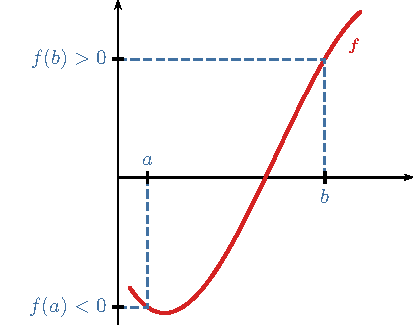
\includegraphics[scale=0.9]{Chapitre_3_analyse_numerique/figures/fig_1/fig_1.pdf}

\fig{Théorème de la valeur intermédiaire.}
\end{minipage}


La continuité ainsi que la condition $f(a)\cdot f(b)<0$ sont essentielles à l'existence d'un zéro dans l'intervalle $[a;b]$. Si l'une ou l'autre de ces hypothèses n'est pas satisfaite, le théorème de la valeur intermédiaire ne peu garantir l'existence d'un zéro dans l'intervalle $[a;b]$.

\vspace{5mm}
\begin{minipage}{0.48\textwidth}
\begin{center}
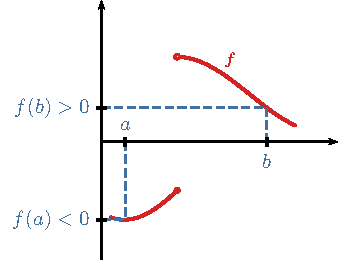
\includegraphics[scale=1]{Chapitre_3_analyse_numerique/figures/fig_2/fig_2.pdf}

\smallskip
\fig{La fonction $f$ n'est pas continue et elle n'admet pas de zéro dans l'intervalle $[a;b]$.}
%\textit{\small La fonction $f$ n'est pas continue et elle n'admet pas de zéro dans l'intervalle $[a;b]$ }
\end{center}
\end{minipage}\hspace{8mm}\begin{minipage}{0.47\textwidth}
\begin{center}
\hspace{-5mm}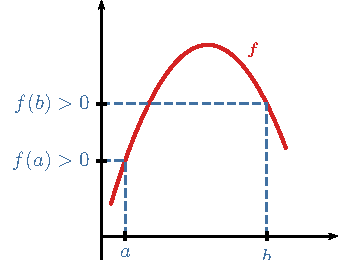
\includegraphics[scale=1]{Chapitre_3_analyse_numerique/figures/fig_3/fig_3.pdf}

\smallskip
\fig{La fonction $f$ ne vérifie pas $f(a)\cdot f(b)<0$ et elle n'admet pas de zéro dans l'intervalle $[a;b]$.}
%\textit{\small La fonction $f$ ne vérifie pas $f(a)\cdot f(b)<0$ et elle n'admet pas de zéro dans l'intervalle $[a;b]$ }
\end{center}
\end{minipage}



\vspace{6mm}
La dichotomie consiste à diviser l'intervalle $[a;b]$ en son milieu puis à \guillemets{détecter} de quel côté du point milieu se situe le zéro. En poursuivant le procédé avec les intervalles suivants, obtenus par répétition de l'opération, on obtient une suite d'intervalles \guillemets{emboités} dont la longueur tend vers 0 et dont les extrémités des intervalles forment 2 suites convergentes vers un zéro de la fonction.


\medskip
Le principe est la suivant : soit $f : [a,b] \to \R$ une fonction continue et telle que $f(a)\cdot f(b)\leqslant 0$.
%\end{minipage}





\begin{itemize}
  \item Si $f(a)\cdot f(\frac{a+b}{2})\le0$, alors il existe
  $c \in [a,\frac{a+b}{2}]$ tel que $f(c)=0$.
  \item Si $f(a)\cdot f(\frac{a+b}{2})>0$ alors
  $f(\frac{a+b}{2})\cdot f(b)\le0$ et donc il existe $c \in [\frac{a+b}{2},b]$ tel que $f(c)=0$.
\end{itemize}


\begin{center}
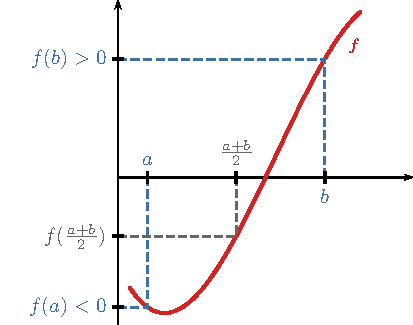
\includegraphics[scale=1]{Chapitre_3_analyse_numerique/figures/fig_4/fig_4.pdf}

\fig{Le zéro se trouve dans la partie droite de l'intervalle $[a;b]$.}
\end{center}


Le nouvel intervalle obtenu contient une solution de l'équation $f(x)=0$ et il a une longueur de moitié par rapport à l'intervalle précédent.


\subsubsection{Le processus algorithmique de la dichotomie}

\begin{itemize}
  \item[] \eh{4.2}{\bf Etape 0 :}\eh{4} On pose $a_0=a$, $b_0=b$. 
  \item[] \eh{4.2}{\bf Etape 1 :}\eh{3}\begin{minipage}[t]{0.8\textwidth}
    $\bullet$  Si $f(a_0)\cdot f(\frac{a_0+b_0}{2}) \le 0$, alors on pose $a_1=a_0$ et $b_1=\frac{a_0+b_0}{2}$,
    
    \smallskip
    $\bullet$ Sinon on pose $a_1=\frac{a_0+b_0}{2}$ et $b_1=b_0$.
 \end{minipage}

  %\item ...
  \item[] {\bf Etape $n+1$ :} \eh{3}\begin{minipage}[t]{0.8\textwidth}
   $\bullet$ Si $f(a_n)\cdot f(\frac{a_n+b_n}{2}) \le 0$, alors on
   pose $a_{n+1}=a_n$ et $b_{n+1}=\frac{a_n+b_n}{2}$,
   
   \smallskip
  $\bullet$ Sinon on pose $a_{n+1}=\frac{a_n+b_n}{2}$ et $b_{n+1}=b_n$.
 \end{minipage}

\end{itemize}

\subsubsection{Justification Mathématique}
L'algorithme décrit ci-dessus permet bien de localiser un zéro de la fonction $f$ prévu par le théorème de la moyenne. C'est ce que démontre le théorème suivant.

\smallskip
\begin{theoreme}[\small \textit{convergence dichotomique}]
Soit $f:[a,b]\to\R$ une fonction continue telle que $f(a)\cdot f(b) \leqslant 0$.\\
Soit également $[a_n;b_n]$ la suite d'intervalles obtenus par le processus dichotomique.

\smallskip
Alors $(a_n)_{n\geqslant 0}$ et $(b_n)_{n\geqslant 0}$ forment deux suites convergentes vers un zéro $c$ de la fonction $f$. 
\end{theoreme}

\smallskip


\begin{demonstration}

A chaque étape de l'algorithme, on obtient deux nombres $a_n$ et $b_n$ tels que :
$$a\leqslant a_{n} \leqslant a_{n+1} \leqslant b_{n+1}\leqslant  b_n \leqslant b$$

%On arrête le processus dès que $b_n-a_n=\frac{b-a}{2^n}$ est inférieur à la précision souhaitée.


Par construction, $(a_n)_{n\in \N}$ et $(b_n)_{n\in \N}$ sont deux suites bornées ainsi que croissante et décroissante respectivement. Donc les deux suites sont convergentes.

\medskip
Par ailleurs, toujours par construction, $(b_n-a_n)=\frac{b-a}{2^n} \to 0$ quand $n\to \infty$ et donc les suites $(a_n)_{n\in \Z}$ \et{1} $(b_n)_{n\in \Z}$ convergent vers la même valeur. 

\medskip
Vu que $a_n\leqslant c\leqslant b_n\eh{2} \forall n\in\N$, on a :
$$\lin{\infty} a_n\leqslant c\leqslant \lin{\infty} b_n$$

\medskip
et comme les suites convergent vers la même valeur alors par le \guillemets{théorème du sandwich}  :
$$\lin{\infty} a_n=c=\lin{\infty} b_n$$

\vspace{-3mm}
\hfill $\blacksquare$
\end{demonstration}




%---------------------------------------------------------------
\subsection{Applications : approximation de  $\sqrt{2}$}

Nous allons utiliser le processus dichotomique pour calculer une valeur approchée de $\sqrt{2}$. Il faut choisir judicieusement la fonction $f$ ainsi que le bornes $a$ et $b$ de l'intervalle.

\medskip
On choisit $f(x)=x^2-2$. C'est une fonction continue sur $\R$ qui s'annule en $\pm\sqrt{2}$ et $\sqrt{2}$ est l'unique solution positive de l'équation $f(x)=0$.

\medskip
Par ailleurs, $f(1) \leqslant 0$ et $f(2) \geqslant 0$, donc l'équation $f(x)=0$ admet une solution dans l'intervalle $[1,2]$. Cette solution est donc nécessairement $\sqrt{2}$.


%Notez que l'on ne choisit pas pour $f$ la fonction $x\mapsto x-\sqrt{2}$ car on ne connaît pas la valeur de $\sqrt{2}$. C'est ce que l'on cherche à calculer !




\begin{enumerate}[label=\arabic*)]
\item On pose $a_0=1$ \et{1} $b_0=2$ \eh{0.2} puis on calcule $\frac{1+2}{2} = 1,5$.
$$f(1,5)=0.25\geqslant 0 \eh{2}\Rightarrow \eh{2} f(1)\cdot f(1,5)\leqslant 0$$
Donc $\sqrt{2}$ est dans l'intervalle $[1 ; 1,5]$.

\item On pose $a_1 = 1$ \et{1} $b_1 = 1,5$ \eh{0.2} puis on calcule $\frac{1+1,5}{2} = 1,25$.
$$f(1,25)=-0,4375 \leqslant 0 \eh{2}\Rightarrow \eh{2} f(1)\cdot f(1,25)\geqslant 0$$
Donc $\sqrt{2}$ est dans l'intervalle $[1,25 ; 1,5]$.

\item On pose $a_2 = 1,25$ \et{1} $b_2 = 1,5$ \eh{0.2} puis on calcule $\frac{1,25+1,5}{2} = 1,375$.
$$f(1,375)=-0,109\ldots \leqslant 0 \eh{2}\Rightarrow \eh{2} f(1,25)\cdot f(1,375)\geqslant 0$$
Donc $\sqrt{2}$ est dans l'intervalle $[1,375 ; 1,5]$.
\end{enumerate}

\begin{center}
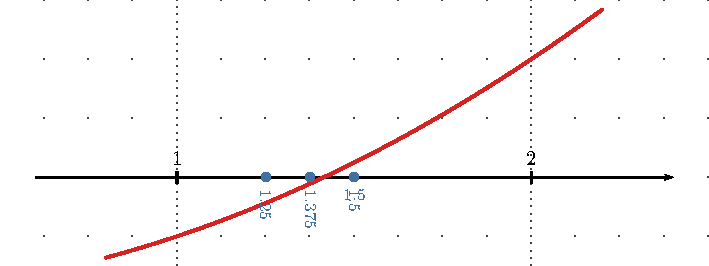
\includegraphics[scale=1]{Chapitre_3_analyse_numerique/figures/fig_5/fig_5.pdf}

\smallskip
\begin{minipage}{0.9\textwidth}
\begin{center}
\fig{On encadre de plus en plus précisément la valeur du zéro positif de la fonction $f(x)=x^2-2$.}
%\textit{\small On encadre de plus en plus précisément la valeur du zéro positif de la fonction $f(x)=x^2-2$ }
\end{center}
\end{minipage}
\end{center}

\smallskip
En poursuivant, on obtient les valeurs suivantes pour les 8 premières étapes :
$$
\begin{array}{ll}
  a_0 = 1			& b_0 = 2 \\
  a_1 = 1			& b_1 = 1,5 \\
  a_2 = 1,25		& b_2 = 1,5 \\
  a_3 = 1,375		& b_3 = 1,5 \\
  a_4 = 1,375		& b_4 = 1,4375 \\
  a_5 = 1,40625		& b_5 = 1,4375 \\
  a_6 = 1,40625		& b_6 = 1,421875 \\
  a_7 = 1,4140625	& b_7 = 1,421875 \\
  a_8 = 1,4140625\eh{3}	& b_8 = 1,41796875 \\
\end{array}
$$

Donc en $8$ étapes on obtient l'encadrement :
$$1,414  \leqslant \sqrt{2} \leqslant 1,417$$

Ce qui permet de déduire les deux premières décimales :
$\sqrt{2}\simeq 1,41$


\bigskip
\begin{boxexstheorieligne}
\begin{enumerate}[label=\textbf{E\thechapter.\arabic*},itemsep=4mm,series=refexercices]
\item En vous inspirant de l'exemple précédent, calculer à la main (calculatrice autorisée) un encadrement au dixième près (première décimale correcte) de $\sqrt{3}$.
\item Selon vous, serait-il plus efficace, d'un point de vue de la complexité de l'algorithme, de diviser les intervalles en 4 plutôt qu'en 2? Justifier votre réponse.
\item Écrire un programme en python qui détermine une approximation des zéros d'une fonction $f$ par la méthode de la dichotomie. On implémentera :
\vspace{-1mm} 
\begin{itemize}
\item une fonction python qui renvoie l'image d'une fonction $f$ donnée ({\small par exemple $f(x)=x^2-2$}).
\item une fonction python \comp{dichotomie\_etape(a,b,n)} qui prend en paramètre les nombres $a$ et $b$ ($a\leqslant b$) ainsi que le nombre d'étapes $n$ désiré.\\
La fonction renvoie les valeurs de $a$ et $b$ à la $n$\up{ième} étape.
\end{itemize}
\item Modifier la fonction \comp{dichotomie\_etape(a,b,n)} de l'exercice précédent pour qu'elle affiche également les valeurs de $a$ et $b$ à chaque étape.
\item\label{dicho_racine_2} En vous aidant de la fonction \comp{dichotomie\_etape(a,b,n)} et en utilisant la fonction définie par $f(x)=x^2-2$ sur l'intervalle $[1;2]$, faire des essais pour plusieurs valeurs de $n$ pour déterminer le nombre d'étapes nécessaires pour obtenir la 5\up{ième} décimale correcte de $\sqrt{2}$.
\item Vérifier que $x=2$ est un zéro de la fonction $f(x)=4x^4-12x^3+x^2+12x+4$.\\
Peut-on appliquer l'algorithme de dichotomie pour déterminer ce zéro ? 
\end{enumerate}
\end{boxexstheorieligne}



%\begin{tikzpicture}[remember picture,overlay]
%\path[left color=orange,right color=white]
%([yshift=-30pt]current page.north west)
%+(0,-2pt) rectangle +(14cm,2pt); 
%
%\path[left color=orange,right color=white]
%([yshift=-175pt,xshift=+14cm]current page.north west)
%+(0,-.5pt) rectangle +(5.1cm,0.5pt);
%\end{tikzpicture}


%%---------------------------------------------------------------
%\subsection{Résultats numériques pour $(1,10)^{1/12}$}
%
%
%Nous cherchons maintenant une approximation de $(1,10)^{1/12}$.
%Soit $f(x) = x^{12} - 1,10$.
%On pose $a_0=1$ et $b_0=1,1$. Alors $f(a_0)=-0,10 \le 0$ et $f(b_0)=2,038\ldots \ge 0$.
%
%$$
%\begin{array}{ll}
%  a_0 = 1             & b_0 = 1,10 \\
%  a_1 = 1             & b_1 = 1,05 \\
%  a_2 = 1             & b_2 = 1,025 \\
%  a_3 = 1             & b_3 = 1,0125 \\
%  a_4 = 1,00625       & b_4 = 1,0125 \\
%  a_5 = 1,00625       & b_5 = 1,00937\ldots\\
%  a_6 = 1,00781\ldots & b_6 = 1,00937\ldots \\
%  a_7 = 1,00781\ldots & b_7 = 1,00859\ldots \\
%  a_8 = 1,00781\ldots & b_8 = 1,00820\ldots \\
%\end{array}
%$$
%
%Donc en $8$ étapes on obtient l'encadrement :
%$$ 1,00781 \le (1,10)^{1/12} \le 1,00821$$



%---------------------------------------------------------------
\subsection{Calcul de l'erreur}

La méthode de dichotomie fournit un encadrement d'un zéro de $f(x)$ et, par construction, la longueur de l'intervalle à l'étape $n$ représente l'erreur maximale commise dans l'estimation du zéro (à l'étape $n$). On appelle cette erreur maximale  la \textbf{précision} de l'approximation du zéro.

\smallskip
Nous remarquons que la précision augmente d'un facteur 2 d'une étape à l'autre car la taille de l'intervalle contenant le zéro est divisée par $2$.

%Au départ, on sait que $\ell \in [a,b]$ (de longueur $b-a$) ;
%puis $\ell  \in [a_1,b_1]$ (de longueur $\frac{b-a}{2}$) ;
%puis $\ell \in [a_2,b_2]$ (de longueur $\frac{b-a}{4}$) ; ... ;
%$[a_n,b_n]$ étant de longueur $\frac{b-a}{2^n}$.

\medskip
Concrètement, si $x_0$ est un zéro de la fonction $f$ dans l'intervalle $[a;b]$, alors on sait que $a_n \leqslant x_0 \leqslant b_n$ et donc $$|x_0-a_n| \leqslant |b_n-a_n| = \frac{b-a}{2^n}$$

Pour obtenir une approximation de $x_0$ avec une précision de $10^{-N}$, il faut choisir $n$ tel que  $\frac{b-a}{2^n} \leqslant 10^{-N}$ :

\setlength{\jot}{3mm}
\hspace*{2cm}\begin{minipage}{0.6\textwidth}\begin{align*}
\frac{b-a}{2^n} \leqslant 10^{-N}
 & \ssi[2] (b-a)10^N \leqslant 2^n  \\
 & \ssi[2] \log(b-a) + \log(10^N)  \leqslant \log(2^n) \\
 & \ssi[2] \log(b-a) + N \leqslant n \log(2) \\
 & \ssi[2] n \geqslant \frac{N +  \log(b-a)}{\log(2)} \\
\end{align*}\end{minipage}

\vspace{-2mm}
Il faut donc que $n \geqslant \frac{N +  \log(b-a)}{\log(2)}$ pour obtenir une précision de $N$ chiffres après la virgule. 
%Sachant $\log(2) \simeq 0,301$, si par exemple $b-a \leqslant 1$, voici le nombre d'itérations suffisantes pour avoir une  précision de $10^{-N}$ (ce qui correspond, à peu près, à $N$ chiffres exacts après la virgule).
%\begin{center}
%\begin{tabular}{ll}
%  $10^{-10}$ ($\sim 10$ décimales) &  $34$ itérations \\
%  $10^{-100}$ ($\sim 100$ décimales) &  $333$ itérations \\
%  $10^{-1000}$ ($\sim 1000$ décimales) &  $3322$ itérations \\
%\end{tabular}
%\end{center}
%
%On remarque qu'il faut entre $3$ et $4$ itérations supplémentaires pour obtenir une nouvelle décimale.

\bigskip
\begin{remarque}
En toute rigueur il ne faut pas confondre précision et nombre de décimales exactes.\\
Par exemple $0,999$ est une approximation de $1$ à $10^{-3}$ près, mais aucune
décimale après la virgule n'est exacte.  En pratique, c'est la précision qui est la plus importante, mais il est plus\\ \guillemets{frappant} de parler du nombre de décimales exactes.
\end{remarque}





\bigskip
\begin{boxexstheorieligne}
\begin{enumerate}[label=\textbf{E\thechapter.\arabic*},itemsep=4mm,resume=refexercices]
\item En supposant $b-a\leqslant 1$, calculer à la main (calculatrice autorisée) le nombre minimum d'étapes qu'il faut effectuer pour obtenir une précision de :
\begin{multicols}{3}
\begin{enumerate}[label=\roman*)]
\item $10^{-10}$ {\footnotesize($\sim 10$ décimales)}
\item $10^{-100}$ {\footnotesize($\sim 100$ décimales)}
\item $10^{-1000}$ {\footnotesize($\sim 1000$ décimales)}
\end{enumerate}
\end{multicols}
\item Avec les même conditions que l'exercice précédent, combien faut-il d'étapes pour gagner une décimale de précision? 
\item\label{dicho_prec} Écrire un programme en python qui détermine une approximation des zéros d'une fonction $f$ par la méthode de la dichotomie avec la précision désirée. On implémentera :
\vspace{-1mm} 
\begin{itemize}
\item une fonction python \comp{dichotomie\_precision(a,b,precision)} qui prend en paramètre les nombres $a$ et $b$ ($a\leqslant b$) ainsi que la \textit{precision} désirée.\\
La fonction renvoie les valeurs de $a$ et $b$.
\end{itemize}
\item Après avoir localisé des intervalles approprié (graphique avec geogebra autorisé), déterminer tous les zéros des fonction suivantes en vous servant du programme de l'exercice \ref*{dicho_prec} :
\begin{multicols}{2}
\begin{enumerate}[label=\roman*)]
\item $f(x)=e^{x-1}-\frac{x^4}{4}$\eh{3} \textit{(précision : $10^{-3}$)}
\item $g(x)=\sin^2(x)+\frac{\phantom{^4}x\phantom{^4}}{3}$\eh{3} \textit{(précision : $10^{-4}$)}
\end{enumerate}
\end{multicols}
%\item Que fait la fonction \comp{mystere} ci-dessous :
%
%\insertcode{Algos/mystere.py}{fonction.py}{0.65}
%\item En vous aidant de la fonction \comp{dichotomie\_etape(a,b,n)} et en faisant des essais pour plusieurs valeurs du nombre d'étapes $n$, déterminer le nombre d'étapes nécessaires pour obtenir une précision de $10^{-5}$ (la 5\up{ième} décimale est correcte) de $\sqrt{2}$.
\end{enumerate}
\end{boxexstheorieligne}



























































%%---------------------------------------------------------------
%\subsection{Algorithmes}
%
%Voici comment implémenter la dichotomie dans le langage Python. Tout d'abord
%on définit une fonction $f$ (ici par exemple $f(x)=x^2-10$) :
%
%%\insertcode{algos/dichotomie-tex1.py}{dichotomie.py (1)}
%
%Puis la dichotomie proprement dite : en entrée de la fonction, on a
%pour variables $a,b$ et $n$ le nombre d'étapes voulues.
%
%%\insertcode{algos/dichotomie-tex2.py}{dichotomie.py (2)}
%
%Même algorithme, mais avec cette fois en entrée la précision souhaitée :
%
%%\insertcode{algos/dichotomie-tex3.py}{dichotomie.py (3)}
%
%
%Enfin, voici la version récursive de l'algorithme de dichotomie.
%
%%\insertcode{algos/dichotomie-tex4.py}{dichotomie.py (4)}
%
%
%%---------------------------------------------------------------
%%\subsection{Mini-exercices}
%
%%\begin{miniexercices}
%\begin{enumerate}
%  \item \`A la main, calculer un encadrement à $0,1$ près de $\sqrt{3}$.
%  Idem avec $\sqrt[3]{2}$.
%
%  \item Calculer une approximation des solutions de l'équation $x^3+1=3x$.
%
%  \item Est-il plus efficace de diviser l'intervalle en $4$ au lieu d'en $2$ ?
%  (\`A chaque itération, la dichotomie classique nécessite l'évaluation de $f$ en une nouvelle valeur
%  $\frac{a+b}{2}$ pour une précision améliorée d'un facteur $2$.)
%
%  \item \'Ecrire un algorithme pour calculer plusieurs solutions de $(f(x)=0)$.
%
%  \item On se donne un tableau trié de taille $N$, rempli de nombres appartenant à $\{1,\ldots,n\}$.
%  \'Ecrire un algorithme qui teste si une valeur $k$ apparaît dans le tableau et en quelle position.
%
%\end{enumerate}
%%\end{miniexercices}
















